% 12 variables in here:
% u_1 = 0.0, h_1 = 10.0, U_1 = 0.0, H_1 = 10.0, u_2 = 0.0, h_2 = 10.0, U_2 = 0.0, H_2 = 10.0, u_3 = 0.0, h_3 = 10.0, U_3 = 0.0, H_3 = 10.0
\begin{figure}[ht]
\centering
  \subfigure[Height and impulse for point $p_1^L$ resp. $p_1^R$] {
    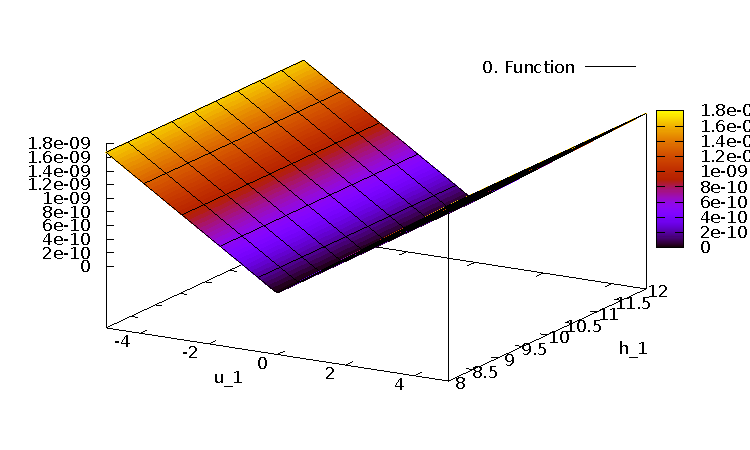
\includegraphics[scale=\zoomfactor]{{{3_punkte_gleich/x_y_0.0_10.0_0.0_10.0_0.0_10.0_0.0_10.0_0.0_10.0f0}}}   
    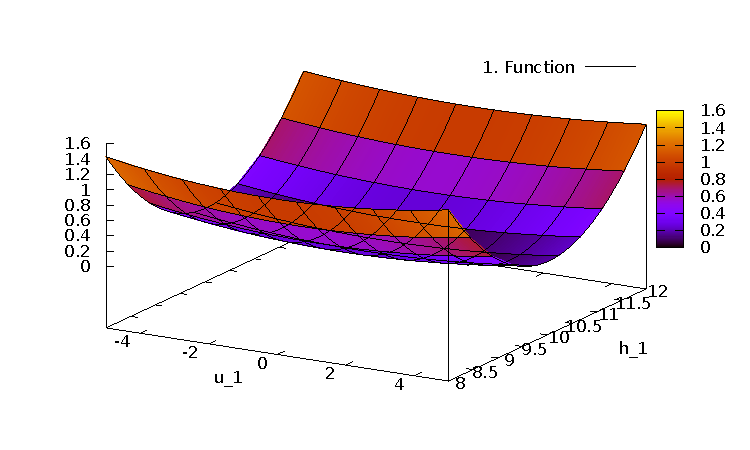
\includegraphics[scale=\zoomfactor]{{{3_punkte_gleich/x_y_0.0_10.0_0.0_10.0_0.0_10.0_0.0_10.0_0.0_10.0f1}}}   
  }

  \subfigure[Height and impulse for point $p_2^L$ resp. $p_2^R$] {
    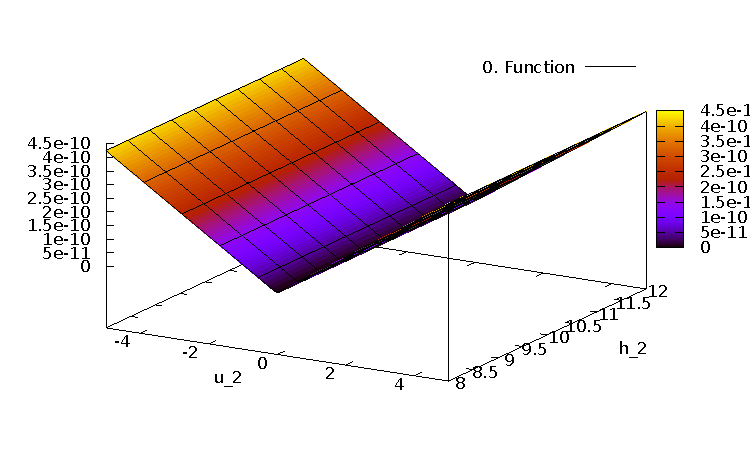
\includegraphics[scale=\zoomfactor]{{{3_punkte_gleich/0.0_10.0_0.0_10.0_x_y_0.0_10.0_0.0_10.0_0.0_10.0f0}}}   
    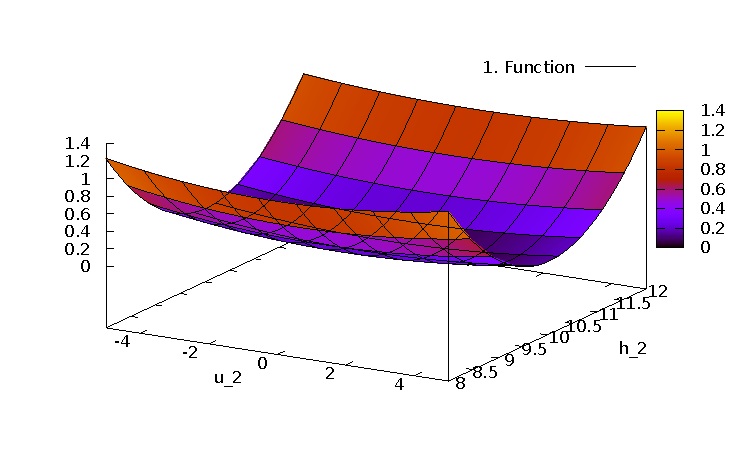
\includegraphics[scale=\zoomfactor]{{{3_punkte_gleich/0.0_10.0_0.0_10.0_x_y_0.0_10.0_0.0_10.0_0.0_10.0f1}}}   
  }

  \subfigure[Height and impulse for point $p_3^L$ resp. $p_3^R$] {    
    {    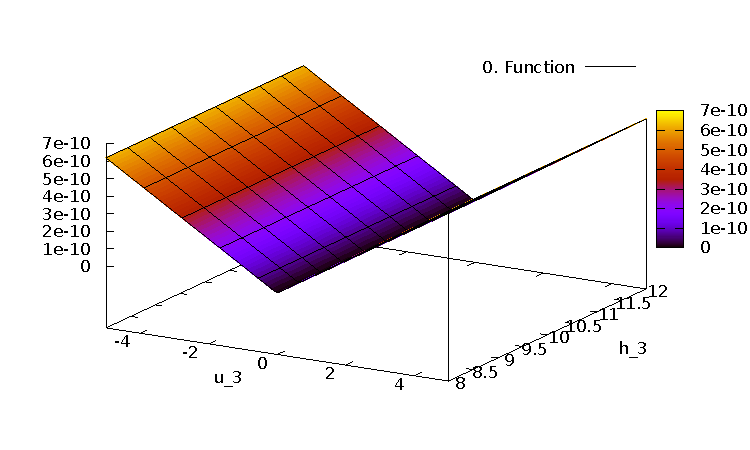
\includegraphics[scale=\zoomfactor]{{{3_punkte_gleich/0.0_10.0_0.0_10.0_0.0_10.0_0.0_10.0_x_y_0.0_10.0f0}}}   }
    {    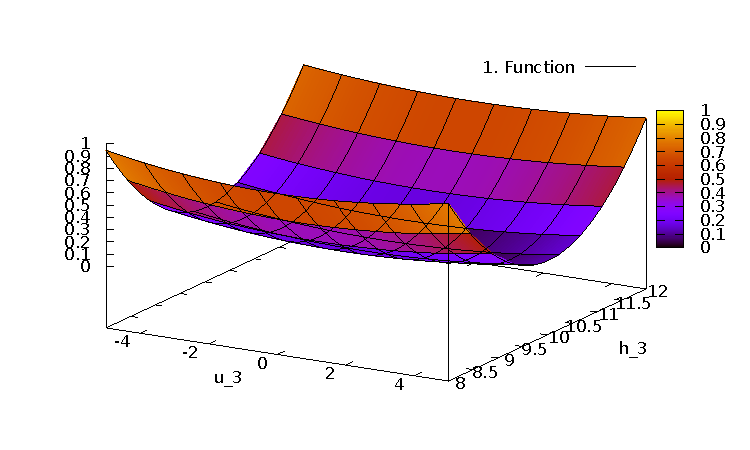
\includegraphics[scale=\zoomfactor]{{{3_punkte_gleich/0.0_10.0_0.0_10.0_0.0_10.0_0.0_10.0_x_y_0.0_10.0f1}}}   }
  }

    % 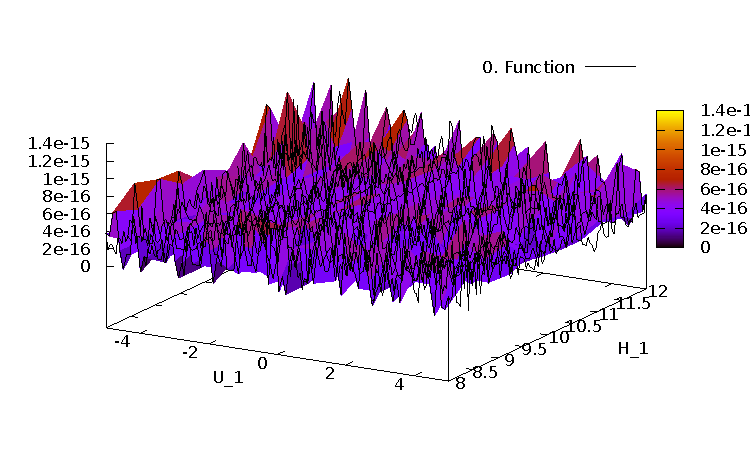
\includegraphics[scale=\zoomfactor]{{{3_punkte_gleich/0.0_10.0_x_y_0.0_10.0_0.0_10.0_0.0_10.0_0.0_10.0f0}}}   
    % 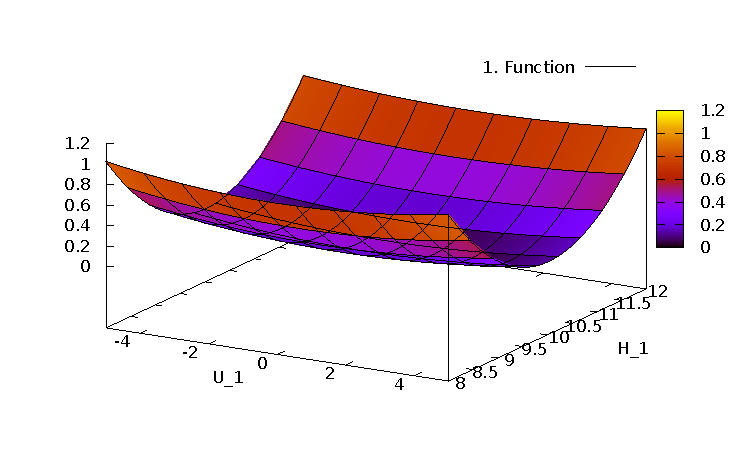
\includegraphics[scale=\zoomfactor]{{{3_punkte_gleich/0.0_10.0_x_y_0.0_10.0_0.0_10.0_0.0_10.0_0.0_10.0f1}}}   
  % \subfigure[] {    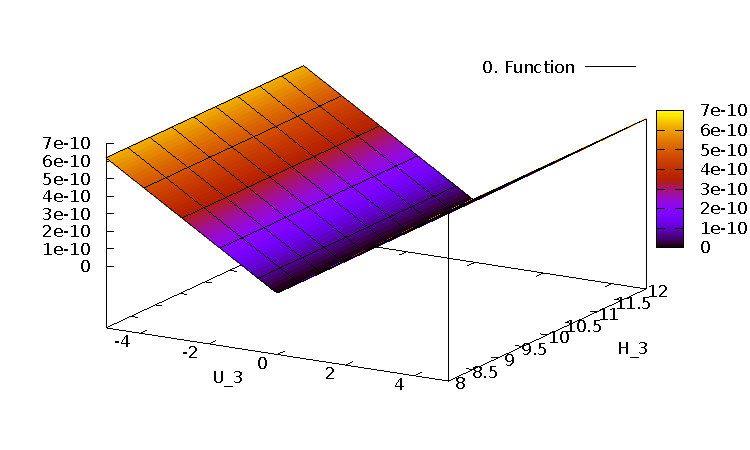
\includegraphics[scale=\zoomfactor]{{{3_punkte_gleich/0.0_10.0_0.0_10.0_0.0_10.0_0.0_10.0_0.0_10.0_x_yf0}}}   }
  % \subfigure[] {    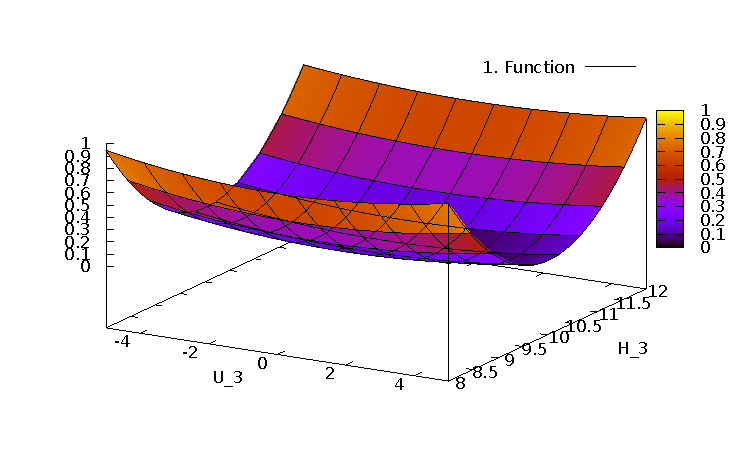
\includegraphics[scale=\zoomfactor]{{{3_punkte_gleich/0.0_10.0_0.0_10.0_0.0_10.0_0.0_10.0_0.0_10.0_x_yf1}}}   }

  % \subfigure[] {    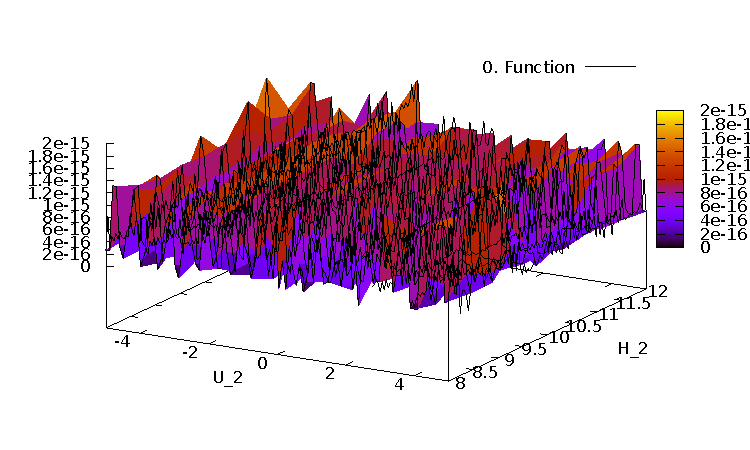
\includegraphics[scale=\zoomfactor]{{{3_punkte_gleich/0.0_10.0_0.0_10.0_0.0_10.0_x_y_0.0_10.0_0.0_10.0f0}}}   }
  % \subfigure[] {    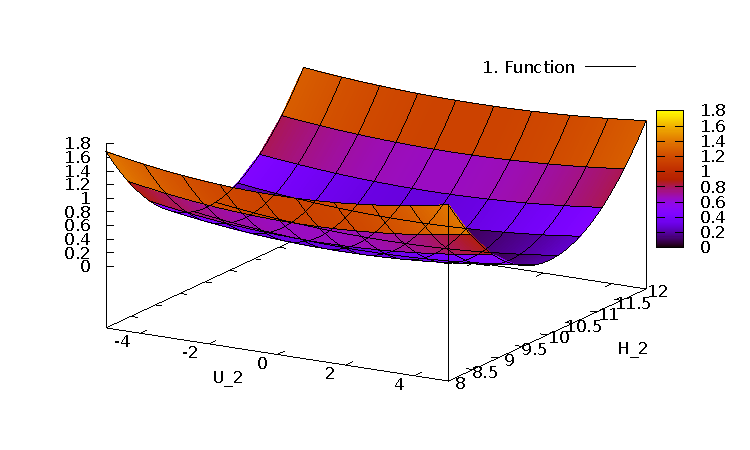
\includegraphics[scale=\zoomfactor]{{{3_punkte_gleich/0.0_10.0_0.0_10.0_0.0_10.0_x_y_0.0_10.0_0.0_10.0f1}}}   }
  \caption{Three points for each triangle. All points have height 10, impulse 0. The remaining points ($P_1, P_2$ and $P_3$) are not plotted since their plots look exactly the same.}
  \label{fig:three-points-equal}
\end{figure}

%%% Local Variables:
%%% TeX-master: "../results.tex"
%%% End:

%%% Local Variables:
%%% TeX-master: "../results.tex"
%%% End:
